Como explanado anteriormente, o motor de passo híbrido congrega características do motor de passo de ímã permanente e o motor de passo de relutância variável. Para entender como o motor de passo híbrido funciona, primeiramente irá ser mostrado brevemente o princípio de funcionamento destes dois outros tipos de motores de passo ora citados, bem como o que são motores de passo, por fim será explicado o funcionamento do motor de passo híbrido em função como um motor aperfeiçoado dos outros dois motores de passo, a fim da explicação se tornar mais familiarizada para o leitor.  

	\subsection{Motor de passo}
	São máquinas elétricas que consistem em um estator com enrolamentos de excitação e um rotor magnético com saliências. Neles o conjugado é produzido pela tendência do rotor a se alinhar com a onda de fluxo produzida pelo estator, de modo a maximizar os fluxos concatenados que resultam da aplicação de uma dada corrente no estator. No motor de passo as fases dos enrolamentos do estator são excitadas sequencialmente, fazendo o rotor girar na forma de uma sequência de passos, com ângulos definidos a cada passo, devido à tendência de alinhamento do rotor com a onda de fluxo do estator. \cite{Fitz} As principais características dos motores de passo são: \cite{MoonsHSM} 
	
	\begin{itemize}
		\item \textbf{Inexistência de escovas:} não necessitam de escovas, reduzindo a maioria das falhas comumente encontradas nos outros motores elétricos, como faiscamento e perdas ôhmicas no rotor e escovas.
		\item \textbf{Independência da carga:} giram com uma dada velocidade independentemente da carga, desde que tal carga não exceda as característica de torque do motor.
		\item \textbf{Menos sensores} se movem com incrementos quantificáveis, desde que com torque especificado, podendo ter conhecimento da posição do eixo.
		\item \textbf{Posição de repouso:} é possível manter o eixo estacionário, desde que seu torque seja respeitado. 
	\end{itemize}
	
	\subsection{Características construtivas gerais do HSM}
	
	Conforme citado anteriormente, o HSM contêm características importantes do VRM e do PMM, o que justifica a denominação 'híbrido'. O estator de um HSM é exatamente um estator do PMM, enquanto que o rotor de um HSM é um rotor do VRM magnetizado.
	
	Como forma de visualizar melhor as duas partes do motor, a Fig. \ref{HSMreal} apresenta o estator e o rotor de um HSM genérico aberto. As especificações deste motor são bem semelhantes ao motor apresentado na Fig. \ref{HSMgrafico}.
	
	\begin{figure}[!h]
		\centering
		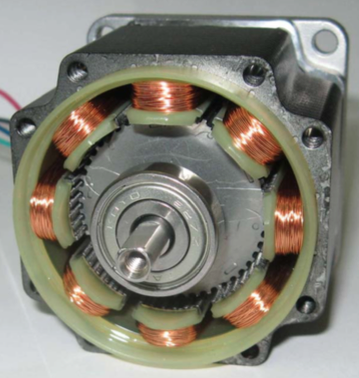
\includegraphics[scale=.45]{Images/hsmreal1.png}
		\caption{Principais partes de um HSM genérico - Visão geral \cite{ieeeRusso}}
		\label{HSMreal}
	\end{figure} 
	
	O estator de um motor de passo híbrido é composto por um dado número de polos magnéticos relacionados com o número de enrolamentos nele, exatamente como em um PMM. Essa característica é herdada dos motores de imã permanente. No PMM, admite-se que para melhorar a resolução de passo, basta adicionar mais enrolamentos ou adicionar mais pares de polos no rotor, através do campo magnético produzido nos enrolamentos deste estator. 
	
	O rotor de um motor de passo híbrido é cuidadosamente seccionado, criando pequenas lacunas chamadas dentes (\textit{teeth}) para gerar uma compensação (\textit{offset}) com relação ao estator para o rotor executar a rotação. É importante citar que o rotor de um HSM é magnetizado, diferentemente do rotor de um VRM.
	
	\begin{figure}[!h]
		\centering
		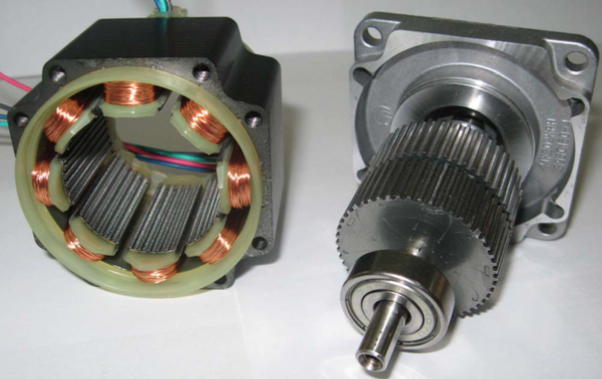
\includegraphics[scale=.4]{Images/hsmreal2.png}
		\caption{Estator (à esquerda) e rotor (à direita) de um HSM genérico \cite{ieeeRusso}}
		\label{HSMestatorrotor}
	\end{figure} 
	
	Verifica-se pela Fig. \ref{HSMestatorrotor} que o estator também é seccionado com alguns dentes. A razão do estator também possuir esses dentes é com o propósito de fazer o motor operar, o que será explanado a seguir.
	
	\subsection{Princípio de funcionamento básico de um motor de passo híbrido}
	
	Conforme pode ser visto na Fig. \ref{HSMestatorrotor}, o rotor de um HSM é seccionado em polos magnéticos que chamaremos de seção sul e seção norte, também denominados \textit{rotor cups}. Essa separação pode ser vista na Fig. \ref{rotorsec}.
	
	\begin{figure}[!h]
		\centering 
		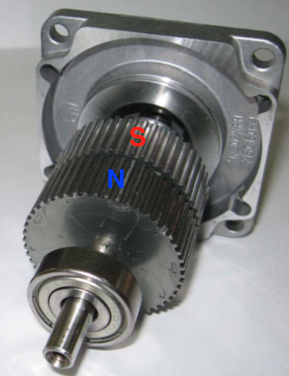
\includegraphics[scale=0.45]{images/hsm_operation/hsmrotorreal}
		\caption{Rotor seccionado em seção sul (S) e seção norte (N) \cite{ieeeRusso}}
		\label{rotorsec}
	\end{figure}
	
	Como apresentado anteriomente e melhor explanado na seção de Características Construtivas do HSM, o rotor é feito com material ferromagnético. De maneira simplificada, apresenta-se o rotor apresentado na Fig. \ref{rotorsec} da seguinte maneira, conforme a Fig. \ref{rotor1}.
	
	\begin{figure}[!h]
		\centering 
		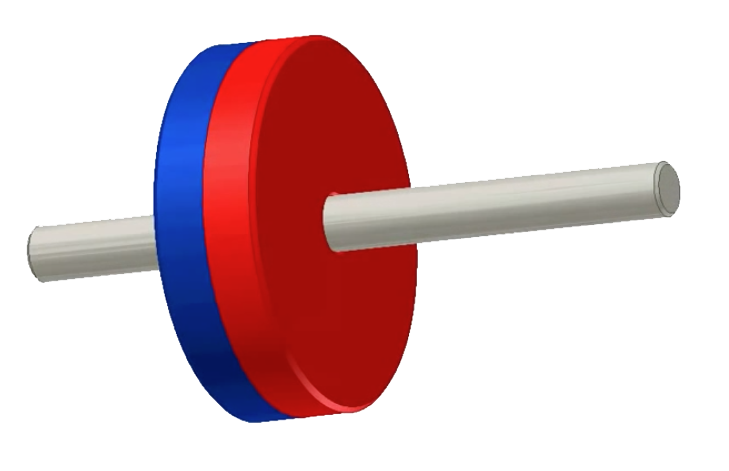
\includegraphics[scale=0.2]{images/hsm_operation/rotormag1}
		\caption{Rotor simplificado de HSM}
		\label{rotor1}
	\end{figure}
	
	Ao rotor mostrado na Fig. \ref{rotor1}, adicionam-se os dentes em cada seção polar, conforme Fig. \ref{rotor2}. O número de dentes determina o número de passo por revolução do motor. Também determina a resolução do passo.
	
	\begin{figure}[!h]
		\centering 
		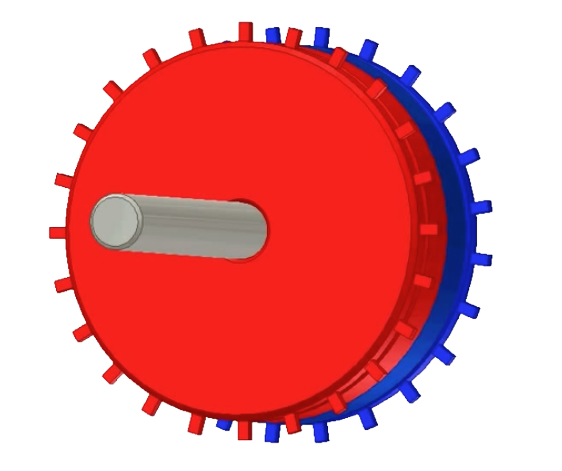
\includegraphics[scale=0.2]{images/hsm_operation/rotormag2}
		\caption{Rotor simplificado de HSM com dentes}
		\label{rotor2}
	\end{figure}
	
	De acordo com a Fig. \ref{rotor3}, verifica-se que os dentes de cada seção polar são espaçados com uma certa compensação devido a alinhação dos dentes. 
	
	\begin{figure}[!h]
		\centering 
		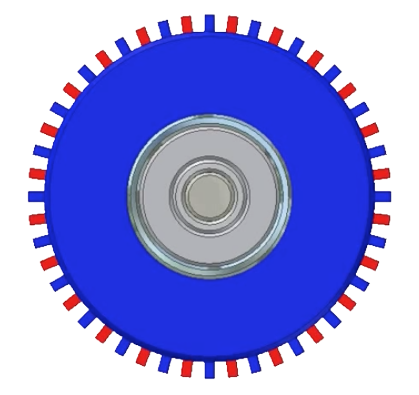
\includegraphics[scale=0.3]{images/hsm_operation/rotormag3}
		\caption{Visão superior do rotor de um HSM}
		\label{rotor3}
	\end{figure}
	
	Essa compensação funciona da seguinte forma: \emph{um dente de uma seção está sempre entre dois dentes da outra seção}. Visualmente, temos a seguinte distribuição de dentes representada na Fig. \ref{rotor4}.
	
	\begin{figure}[!h]
		\centering 
		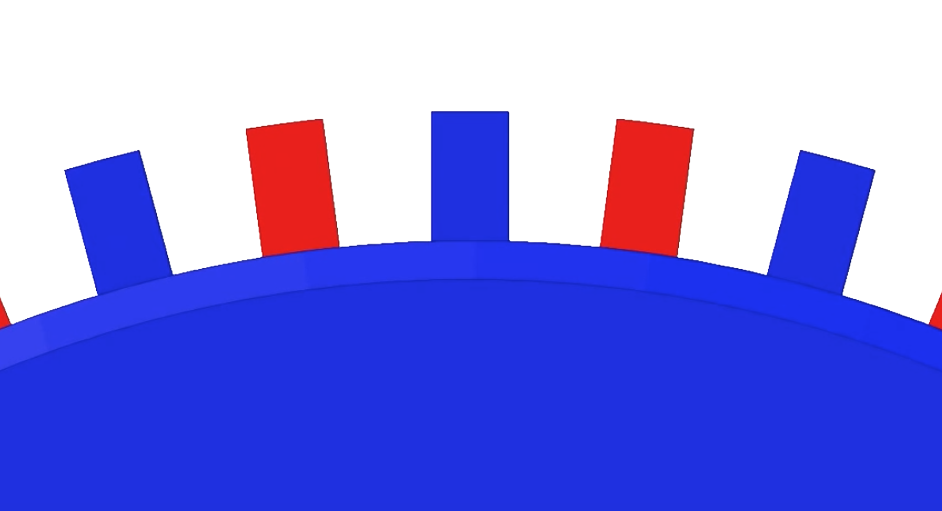
\includegraphics[scale=0.2]{images/hsm_operation/rotormag4}
		\caption{Visão superior do espaçamento entre os dentes das seções do rotor}
		\label{rotor4}
	\end{figure}
	
	Considerando um estator simples de duas fases com quatro enrolamentos, insere-se os enrolamentos na expressão gráfica apresentada anteriormente na Fig. \ref{rotor3}. O HSM simplificado para fins de explicação está representado na Fig \ref{hsm_superior}. 
	
	 \begin{figure}[!h]
		\centering 
		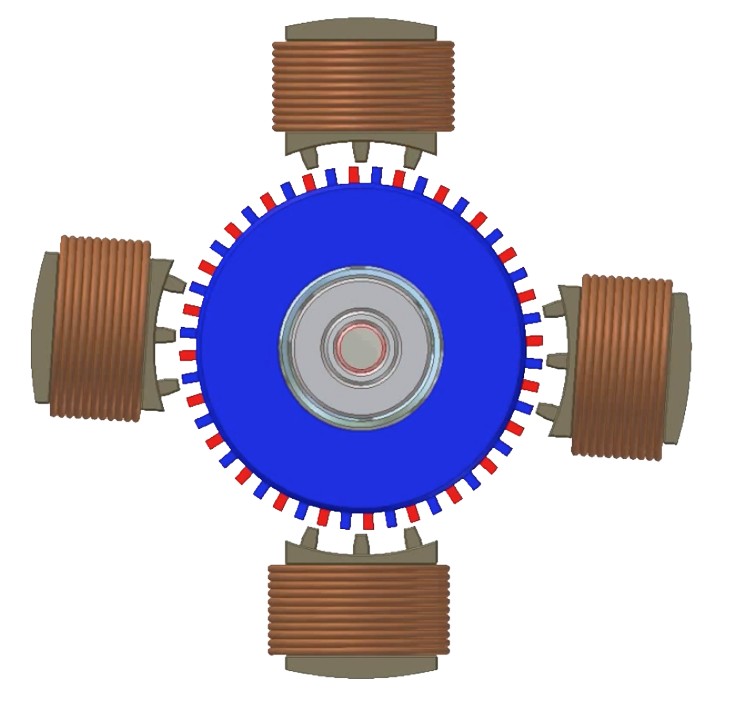
\includegraphics[scale=0.3]{images/hsm_operation/etapa1}
		\caption{Visão superior de um HSM com estator e rotor}
		\label{hsm_superior}
	\end{figure}
	
	
	